\documentclass[aspectratio=169]{beamer}
% nếu dùng tiếng Việt
%\usepackage[utf8x]{vietnam}
\usepackage[T5]{fontenc}
\usepackage{lipsum}

\usetheme{hust}

%\supervisorname{Supervisor:~}
\title{Number Factorization Diagram}

\begin{document}
\section{Backend}
\begin{frame}[noframenumbering,Title]
	\maketitle 
\end{frame}

\begin{frame}{Contents}
	\tableofcontents 
\end{frame}

\begin{frame}[fragile=singleslide]{Backend}
	Fonctions de factorisation :
	\begin{itemize}
		\item Fermat 
		\item Wilson
	\end{itemize}
	\end{frame}
	\begin{frame}[fragile=singleslide]{Méthode de factorisation de Fermat \qquad \qquad \qquad - Sidy SOW -}
	Tout entier naturel se décompose de la difference de deux carrés.\\
	Exemple pour N=14 la fonction renvoi [2,7]
\begin{center}
    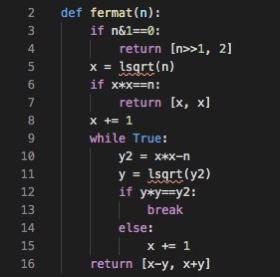
\includegraphics[scale=0.7]{ferma.jpg}
    \end{center}
\end{frame}
\begin{frame}[fragile=singleslide]{Méthode de factorisation de Wilson \qquad \qquad \qquad - Sidy SOW -}
\begin{center}
    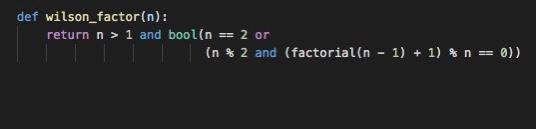
\includegraphics[scale=0.5]{wilson.jpg}
\end{center}
\end{frame}

\begin{frame}[fragile=singleslide]{Backend}
	Implémentation des méthodes de factorisation :
	\begin{itemize}
		\item Facteurs premiers
		\item Pollard Rho
	\end{itemize}
	Implémentation des générateurs des diagrammes de factorisation :
	\begin{itemize}
		\item Pour un entier
		\item Pour une liste d'entiers $\Rightarrow$ \textbf{Poster des diagrammes}
	\end{itemize}
\end{frame}

\begin{frame}[fragile=singleslide]{méthodes de factorisation \qquad \qquad \qquad - Bouthayna HAYOU -}
\begin{center}
    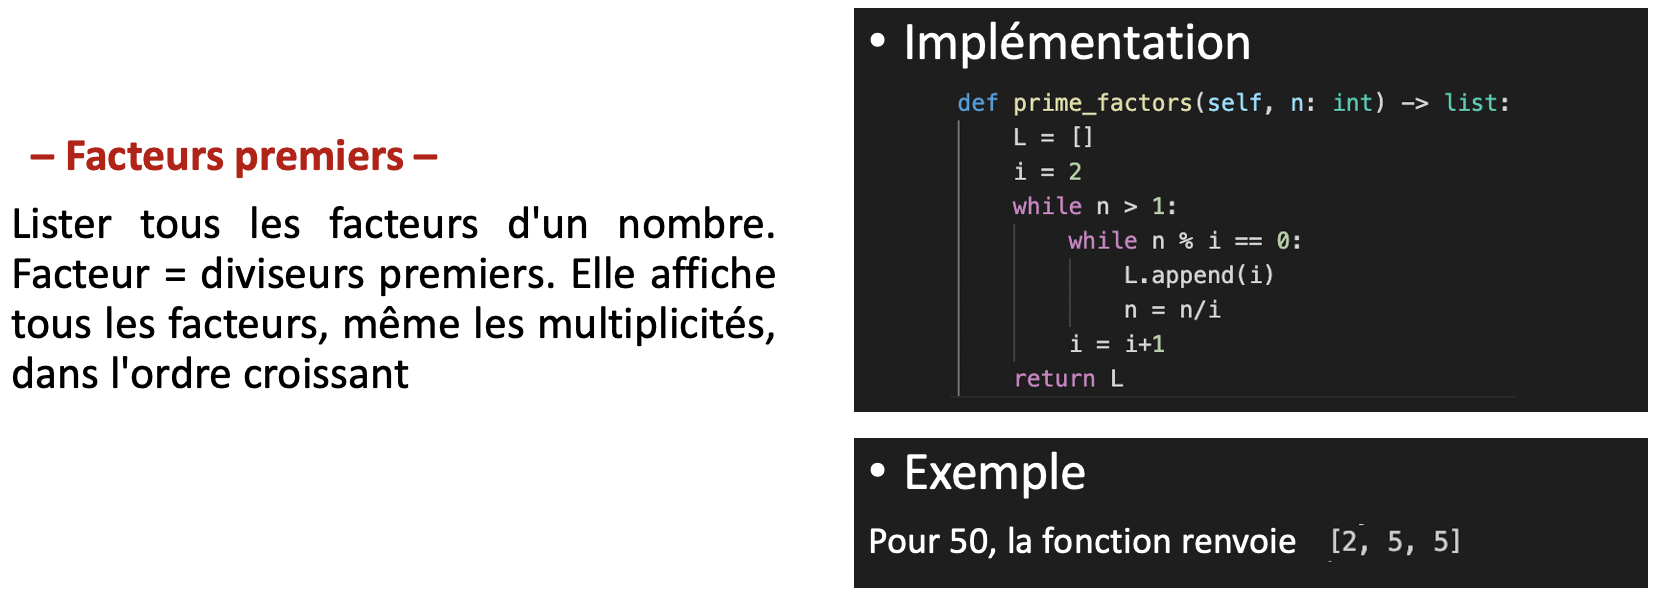
\includegraphics[width=14 cm]{./res/pf.png}
\end{center}
\end{frame}

\begin{frame}[fragile=singleslide]{méthodes de factorisation \qquad \qquad \qquad - Bouthayna HAYOU -}
\begin{center}
    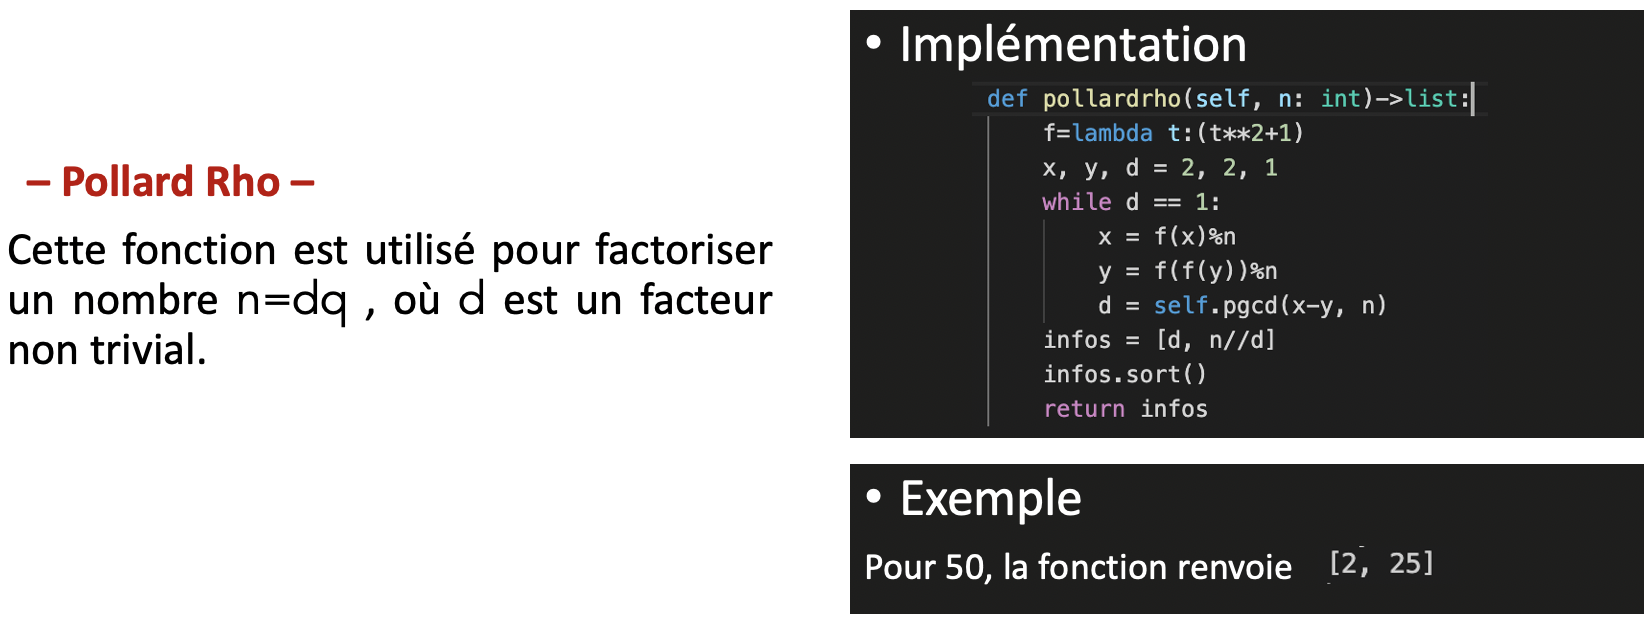
\includegraphics[width=14 cm]{./res/pr.png}
\end{center}
\end{frame}

\begin{frame}[fragile=singleslide]{générateur de diagrammes \qquad \qquad \qquad - Bouthayna HAYOU -}
\begin{center}
    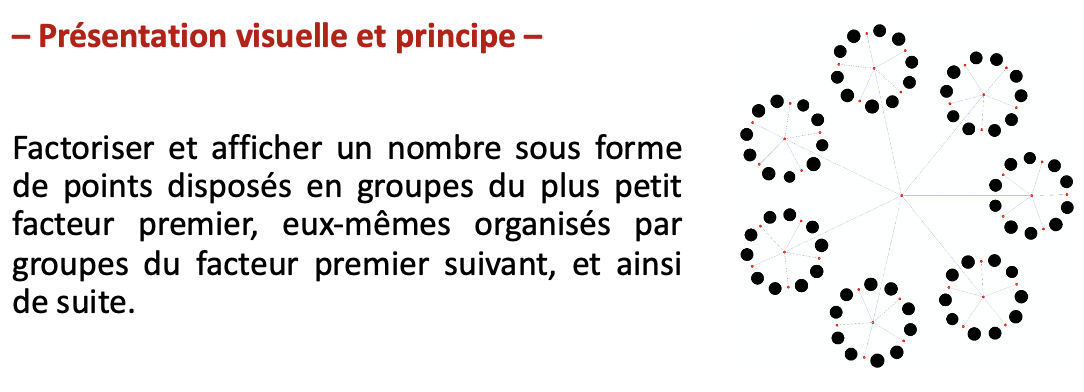
\includegraphics[width=14 cm]{./res/presprincipe.png}
\end{center}
\end{frame}

\begin{frame}[fragile=singleslide]{générateur de diagrammes \qquad \qquad \qquad - Bouthayna HAYOU -}
\begin{center}
    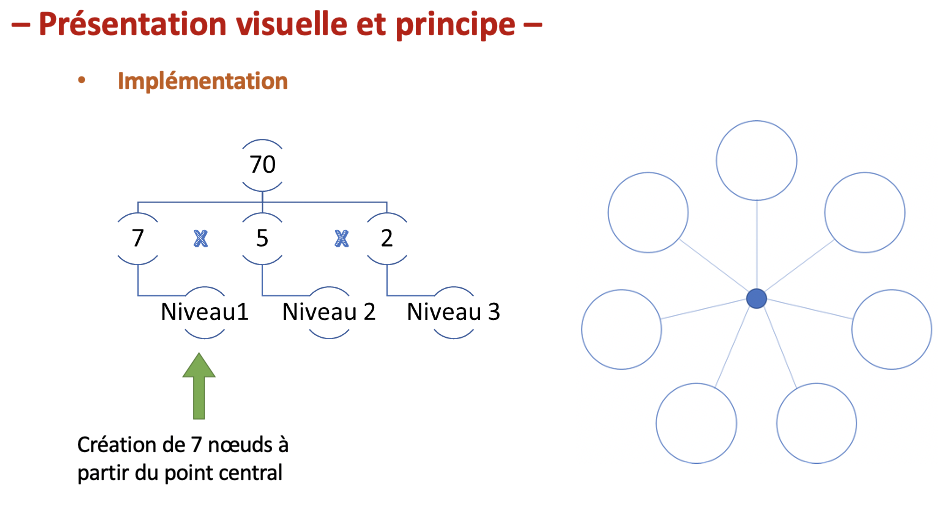
\includegraphics[width=13 cm]{./res/impl1.png}
\end{center}
\end{frame}

\begin{frame}[fragile=singleslide]{générateur de diagrammes \qquad \qquad \qquad - Bouthayna HAYOU -}
\begin{center}
    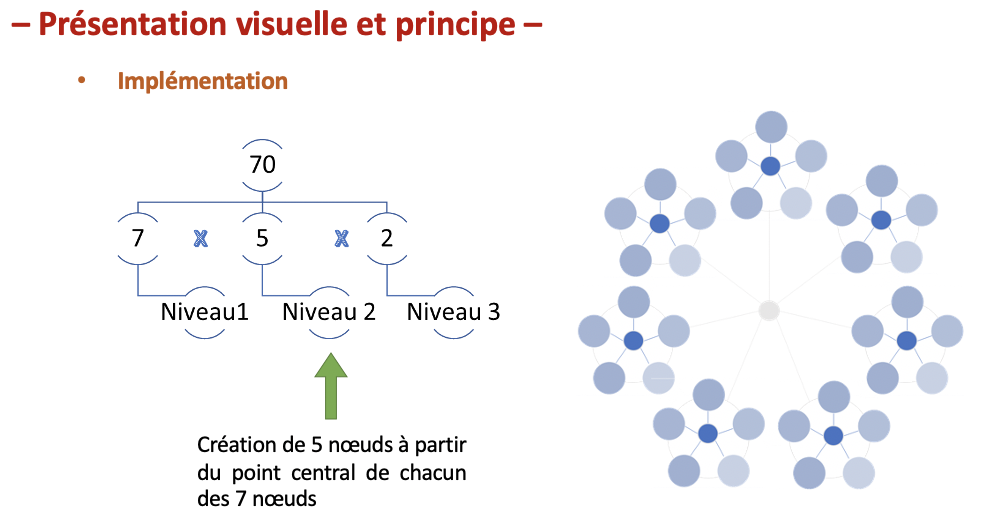
\includegraphics[width=13.5 cm]{./res/impl2.png}
\end{center}
\end{frame}

\begin{frame}[fragile=singleslide]{générateur de diagrammes \qquad \qquad \qquad - Bouthayna HAYOU -}
\begin{center}
    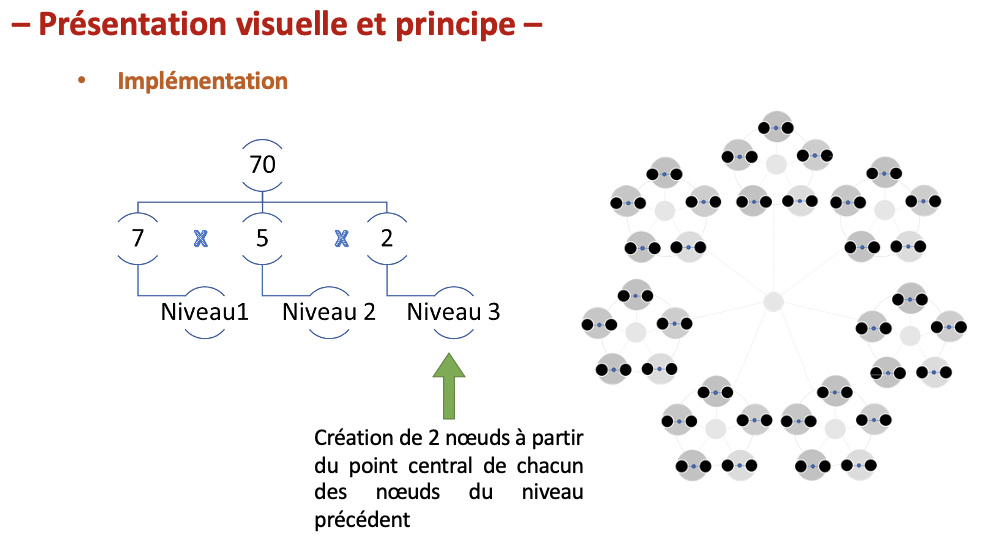
\includegraphics[width=13.5 cm]{./res/impl3.png}
\end{center}
\end{frame}

\begin{frame}[fragile=singleslide]{générateur de diagrammes \qquad \qquad \qquad - Bouthayna HAYOU -}
\begin{center}
    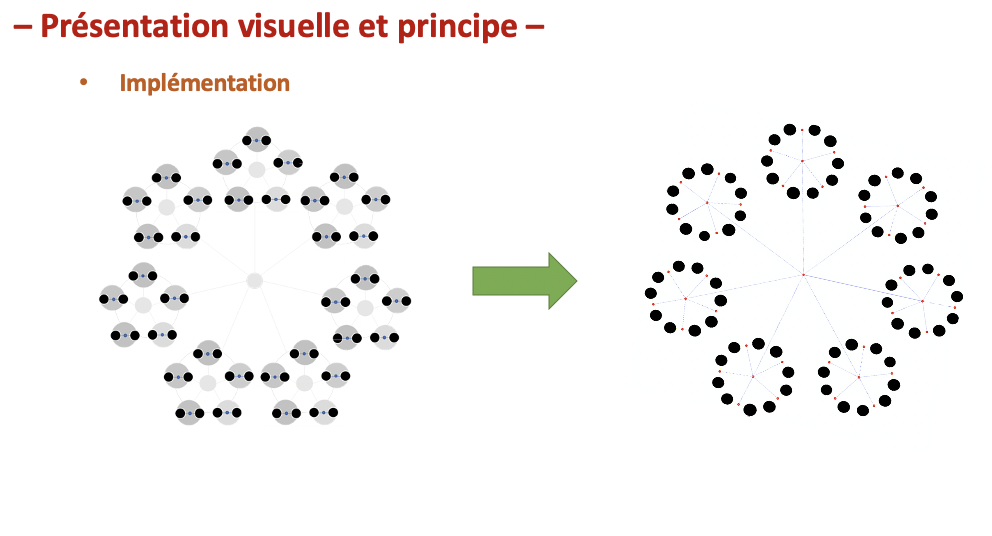
\includegraphics[width=14 cm]{./res/impl4.png}
\end{center}
\end{frame}

\begin{frame}[fragile=singleslide]{générateur du poster \qquad \qquad \qquad \qquad - Bouthayna HAYOU -}
\begin{center}
    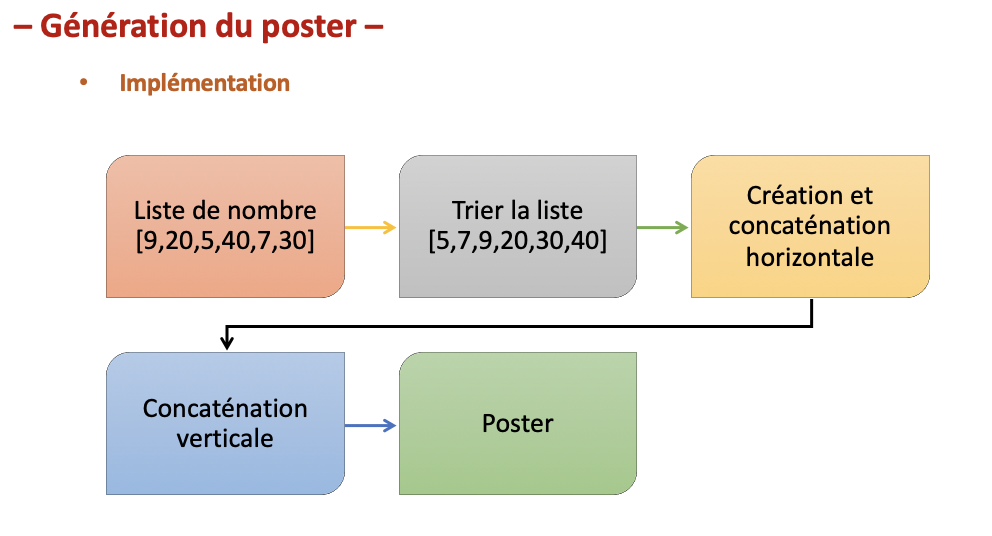
\includegraphics[width=14 cm]{./res/post.png}
\end{center}
\end{frame}

\begin{frame}[fragile=singleslide]{générateur du poster \qquad \qquad \qquad \qquad - Bouthayna HAYOU -}
\begin{center}
    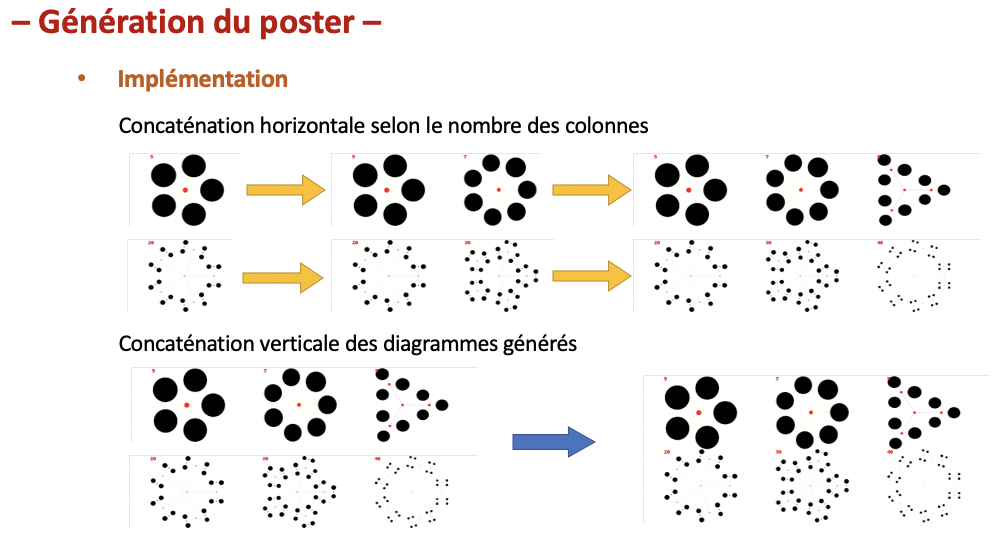
\includegraphics[width=14 cm]{./res/post2.png}
\end{center}
\end{frame}

\begin{frame}[fragile=singleslide]{générateur du poster \qquad \qquad \qquad \qquad - Bouthayna HAYOU -}
\begin{figure}[htp]
\centering
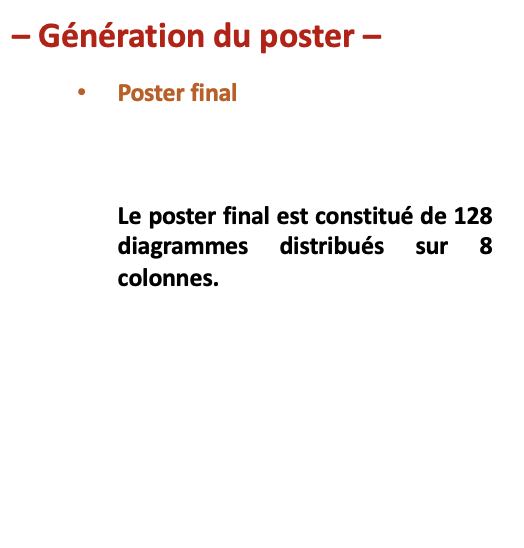
\includegraphics[width=7 cm]{./res/text.png}\hfill
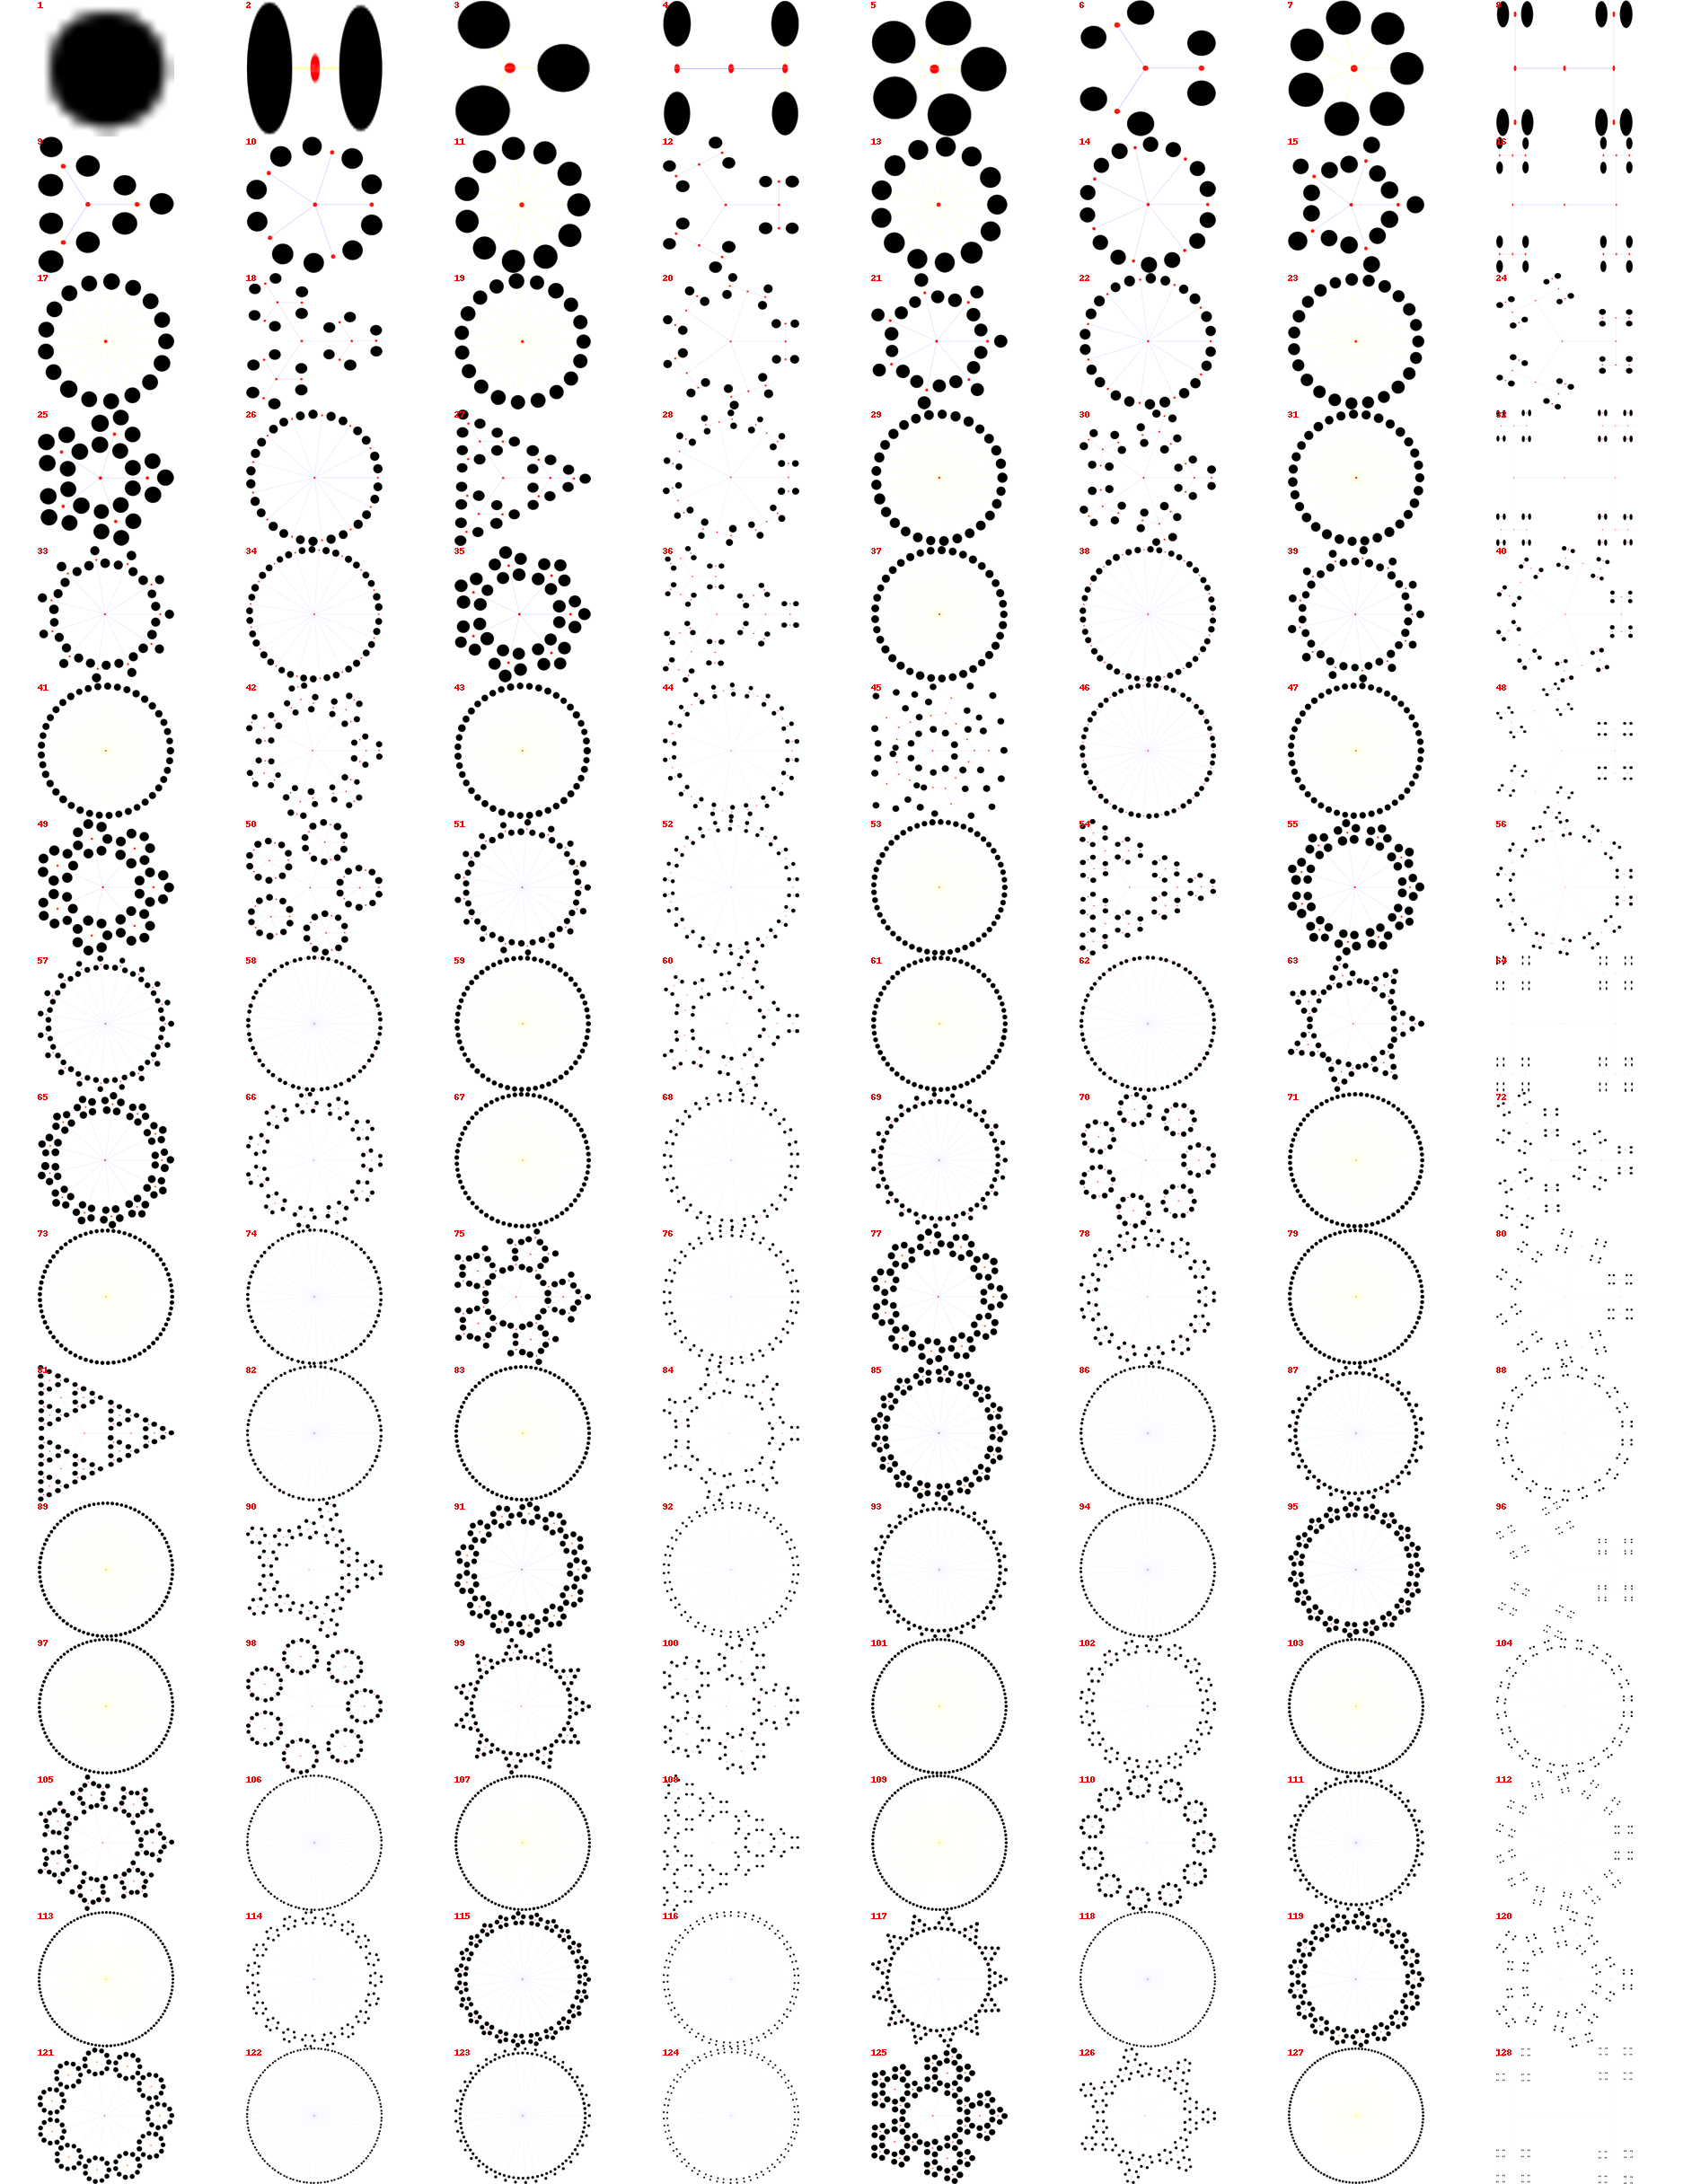
\includegraphics[width=6 cm]{./res/poster.png}
\caption{default}
\label{fig:figure3}
\end{figure}
\end{frame}

\section{Frontend}

\begin{frame}[fragile=singleslide]{FRONTEND}
    Création et affichage des points
    \begin{itemize}
        \item Positions des points 
        \item Création des couleurs
        \item Transitions
    \end{itemize}
    Création de l'animation 
    \begin{itemize}
        \item Fenêtre graphique
        \item Boutons
        \item Texte
    \end{itemize}
\end{frame}

\begin{frame}[fragile=singleslide]{Création des points \qquad \qquad \qquad \qquad \qquad \qquad \qquad - Juliette Lidoine -}
    \begin{center}
        \includegraphics[width=13.5 cm]{./res/pospoints1.pdf}
    \end{center}
\end{frame}

\begin{frame}[fragile=singleslide]{Création des points \qquad \qquad \qquad \qquad \qquad \qquad \qquad - Juliette Lidoine -}
    \begin{center}
        \includegraphics[width=13.5 cm]{./res/pospoints2.pdf}
    \end{center}
\end{frame}

\begin{frame}[fragile=singleslide]{Création des points \qquad \qquad \qquad \qquad \qquad \qquad \qquad - Juliette Lidoine -}
    \begin{center}
        \includegraphics[width=13.5 cm]{./res/pospoints3.pdf}
    \end{center}
\end{frame}

\begin{frame}[fragile=singleslide]{Création des points \qquad \qquad \qquad \qquad \qquad \qquad \qquad - Juliette Lidoine -}
    \begin{center}
        \includegraphics[width=13.5 cm]{./res/pospoints4.pdf}
    \end{center}
\end{frame}

\begin{frame}[fragile=singleslide]{Création des points \qquad \qquad \qquad \qquad \qquad \qquad \qquad - Juliette Lidoine -}
    \begin{center}
        \includegraphics[width=13.5 cm]{./res/pospoints5.pdf}
    \end{center}
\end{frame}

\begin{frame}[fragile=singleslide]{Création des points \qquad \qquad \qquad \qquad \qquad \qquad \qquad - Juliette Lidoine -}
    \begin{center}
        \includegraphics[width=13.5 cm]{./res/pospoints6.pdf}
    \end{center}
\end{frame}

\begin{frame}[fragile=singleslide]{Création des points \qquad \qquad \qquad \qquad \qquad \qquad \qquad - Juliette Lidoine -}
    \begin{center}
        \includegraphics[width=13.5 cm]{./res/couleurs.pdf}
    \end{center}
\end{frame}

\begin{frame}[fragile=singleslide]{Affichage des points \qquad \qquad \qquad \qquad \qquad \qquad \qquad - Louis Nguyen -}
    \begin{center}
        \includegraphics[width=13.5 cm]{./res/transitions1.pdf}
    \end{center}
\end{frame}


\begin{frame}[fragile=singleslide]{Affichage des points \qquad \qquad \qquad \qquad \qquad \qquad \qquad - Louis Nguyen -}
    \begin{center}
        \includegraphics[width=13.5 cm]{./res/transitions2.pdf}
    \end{center}
\end{frame}


\begin{frame}[fragile=singleslide]{Affichage des points \qquad \qquad \qquad \qquad \qquad \qquad \qquad - Louis Nguyen -}
    \begin{center}
        \includegraphics[width=13.5 cm]{./res/affpoints.pdf}
    \end{center}
\end{frame}


\begin{frame}[fragile=singleslide]{Création de l'animation \qquad \qquad \qquad \qquad \qquad \qquad - Louis Nguyen -}
    \begin{center}
        \includegraphics[width=13.5 cm]{./res/statut1.pdf}
    \end{center}
\end{frame}

\begin{frame}[fragile=singleslide]{Création de l'animation \qquad \qquad \qquad \qquad \qquad \qquad - Louis Nguyen -}
    \begin{center}
        \includegraphics[width=13.5 cm]{./res/statut2.pdf}
    \end{center}
\end{frame}

\begin{frame}[fragile=singleslide]{Création de l'animation \qquad \qquad \qquad \qquad \qquad \qquad - Louis Nguyen -}
    \begin{center}
        \includegraphics[width=13 cm]{./res/afftxt1.pdf}
    \end{center}
\end{frame}

\begin{frame}[fragile=singleslide]{Création de l'animation \qquad \qquad \qquad \qquad \qquad \qquad - Louis Nguyen -}
    \begin{center}
        \includegraphics[width=13 cm]{./res/afftxt2.pdf}
    \end{center}
\end{frame}

\begin{frame}[fragile=singleslide]{Création de l'animation \qquad \qquad \qquad \qquad \qquad \qquad - Louis Nguyen -}
    \begin{center}
        \includegraphics[width=13.5 cm]{./res/afftxt3.pdf}
    \end{center}
\end{frame}

\end{document}
